\documentclass[twocolumn,a4j]{jsarticle}
\setlength{\topmargin}{-20.4cm}
\setlength{\oddsidemargin}{-10.4mm}
\setlength{\evensidemargin}{-10.4mm}
\setlength{\textwidth}{18cm}
\setlength{\textheight}{26cm}

\usepackage[top=15truemm,bottom=20truemm,left=20truemm,right=20truemm]{geometry}
\usepackage[latin1]{inputenc}
\usepackage{amsmath}
\usepackage{amsfonts}
\usepackage{amssymb}
\usepackage[dvipdfmx]{graphicx}
\usepackage[hang,small,bf]{caption}
\usepackage[subrefformat=parens]{subcaption}
\usepackage[dvipdfmx]{color}
\usepackage{listings}
\usepackage{listings,jvlisting}
\usepackage{geometry}
\usepackage{framed}
\usepackage{color}
\usepackage[dvipdfmx]{hyperref}
\usepackage{ascmac}
\usepackage{enumerate}
\usepackage{tabularx}
\usepackage{cancel}
\usepackage{scalefnt}
\usepackage{overcite}
\usepackage{otf}
\usepackage{multicol}

\renewcommand{\figurename}{Fig.}
\renewcommand{\tablename}{Table }

\lstset{
basicstyle={\ttfamily},
identifierstyle={\small},
commentstyle={\smallitshape},
keywordstyle={\small\bfseries},
ndkeywordstyle={\small},
stringstyle={\small\ttfamily},
frame={tb},
breaklines=true,
columns=[l]{fullflexible},
xrightmargin=0zw,
xleftmargin=3zw,
numberstyle={\scriptsize},
stepnumber=1,
numbersep=1zw,
lineskip=-0.5ex
}

% キャプション後ろのダブルコロンを消す
\makeatletter
\long\def\@makecaption#1#2{%
  \vskip\abovecaptionskip
  \iftdir\sbox\@tempboxa{#1\hskip1zw#2}%
    \else\sbox\@tempboxa{#1 #2}%
  \fi
  \ifdim \wd\@tempboxa >\hsize
    \iftdir #1\hskip1zw#2\relax\par
      \else #1 #2\relax\par\fi
  \else
    \global \@minipagefalse
    \hbox to\hsize{\hfil\box\@tempboxa\hfil}%
  \fi
  \vskip\belowcaptionskip}
\makeatother

% タイトル
\makeatletter
\def\@maketitle
{
\begin{center}
{\LARGE \@title \par}
\end{center}
\begin{flushright}
{\large \@date 報告書 No.26}\\
{\large M2 \@author}
\end{flushright}
\par\vskip 1.5em
}
\makeatother

\author{来代 勝胤}
\title{令和4年度 4月 第3週 報告書}
\date{2022/4/18}

\begin{document}
\columnseprule=0.1mm
\maketitle

\section*{報告内容}
\begin{enumerate}[1.]
  \item 数値シミュレーションの作成(続)
  \item 正解値の作成と誤差評価
  \item 今後の予定
\end{enumerate}

\section*{進捗状況}
先週に引き続き,
数値シミュレーションの作成と
計測アルゴリズムの適用を行った.
また,計測アルゴリズムの性能評価を行った.

\section{数値シミュレーションの作成(続)}
数値シミュレーションの作成を行うにあたり,
実際の実験条件を再現できるよう,
主流速度及び回転量を参考にして
パラメータの調整を行った.
一部,現実的でない数値があるが
主流速度と各種LLSのパラメータの比から
算出された値を使用している.\\

\subsection{シミュレーション条件}
\begin{table}[hbtp]
  \label{table:data_type}
  \caption{シミュレーション条件}
  \centering
  \begin{tabular}{ c c | r l}
    \hline
    粒子数                  & $n$        & 150000                 & [個]               \\ \hline
    壁の回転速度            & $\omega$   & 10                     & [deg/s]            \\ \hline
    動粘性係数              & $\nu$      & $1.004 \times 10^{-6}$ & [$\mathrm{m}^2$/s] \\ \hline
    $\mathrm{LLS}_1$ の位置 & $x_0$      & 7.000                  & [mm]               \\ \hline
    $\mathrm{LLS}_1$ の厚み & $T_1$      & $3.086\times 10^{-3}$  & [mm]               \\ \hline
    $\mathrm{LLS}_2$ の厚み & $T_2$      & $9.259\times 10^{-3}$  & [mm/s]             \\ \hline
    LLS 間の距離            & $\Delta T$ & $9.645\times 10^{-3}$  & [mm/s]             \\ \hline
  \end{tabular}
\end{table}

\begin{table}[hbtp]
  \label{table:data_type}
  \caption{実験条件(参考)}
  \centering
  \begin{tabular}{ c c | r l}
    \hline
    主流速度       & $u$        & 250   & [mm/s] \\ \hline
    LLS (1) の厚み & $T_1$      & 1.000 & [mm/s] \\ \hline
    LLS (2) の厚み & $T_2$      & 3.000 & [mm/s] \\ \hline
    LLS 間の距離   & $\Delta T$ & 3.125 & [mm/s] \\ \hline
  \end{tabular}
\end{table}

\newpage
\subsection{数値シミュレーションの解析プログラム適用結果}
数値シミュレーションの画像を用いて
解析プログラムの適用結果を Fig.1 に示す.
回転中心は $(y,z) = (400, 200)$ に位置しており,
反時計回りの渦構造を確認することができる.
所々に誤ベクトルが存在するが,
トラッキング時に異なる粒子像とマッチングしてしまうためである.

\begin{figure}[htbp]
  \footnotesize
  \begin{center}
    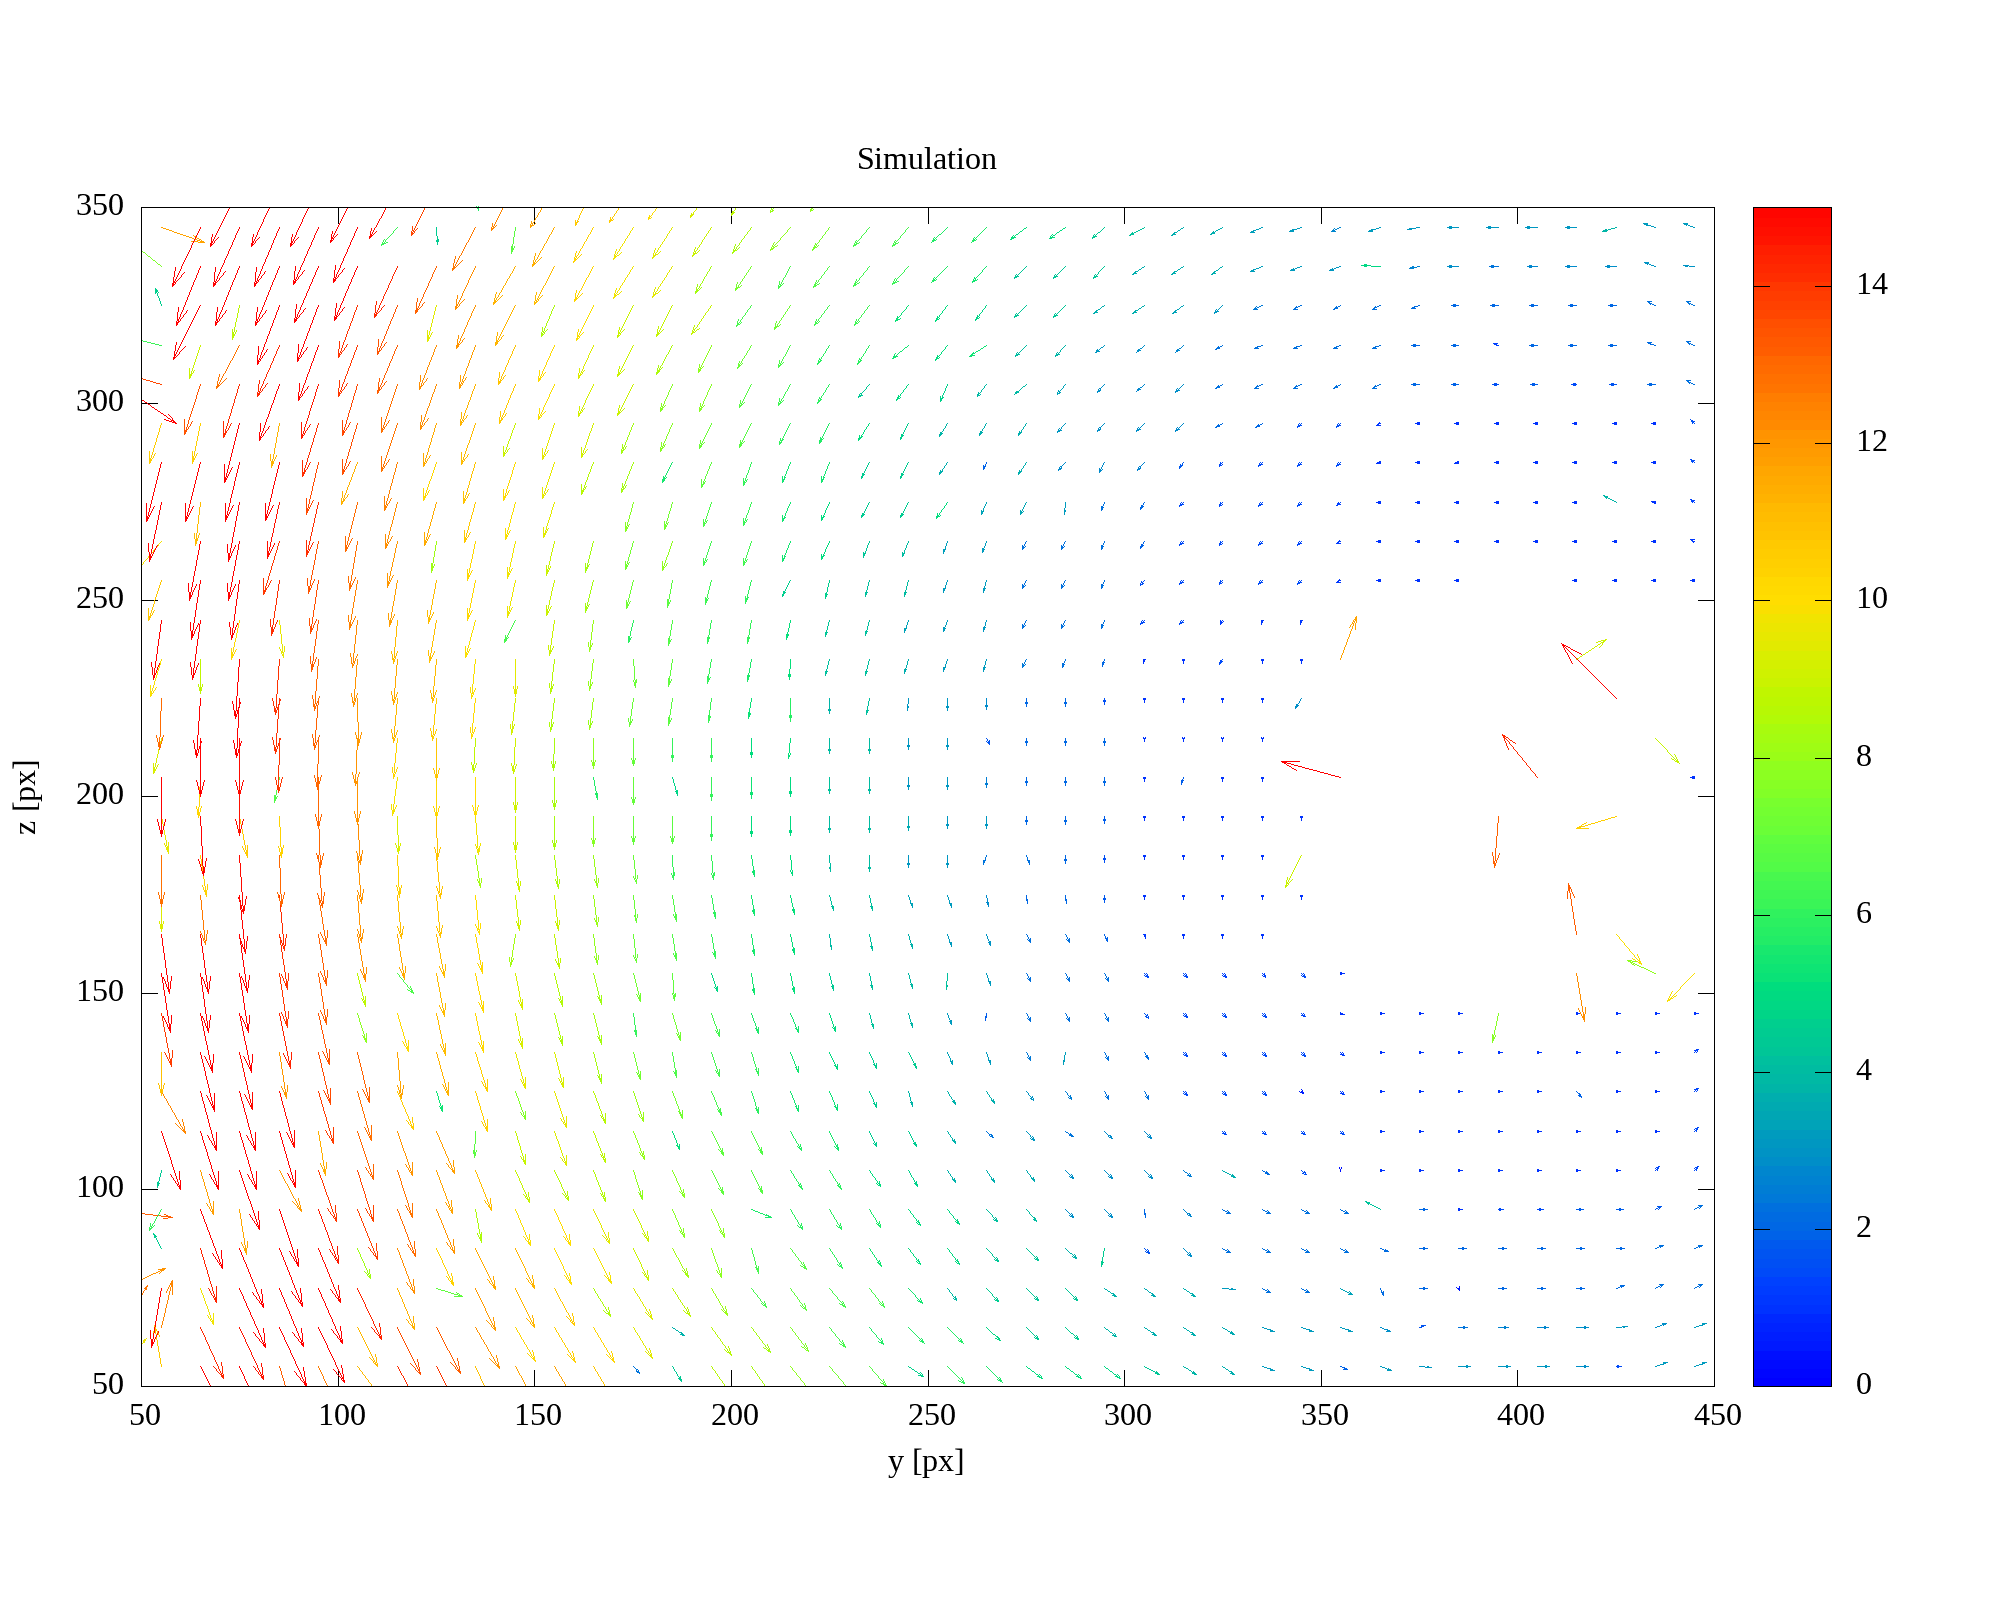
\includegraphics[width=80mm]{../images/average.png}
    \caption{PIV:Simulation}
  \end{center}
\end{figure}

\section{正解値の作成と誤差評価}
解析アルゴリズムの精度評価のため,正解値と比較を行う.
正解値はLLS間の中間位置を基準に作成した.

\begin{figure}[htbp]
  \footnotesize
  \begin{center}
    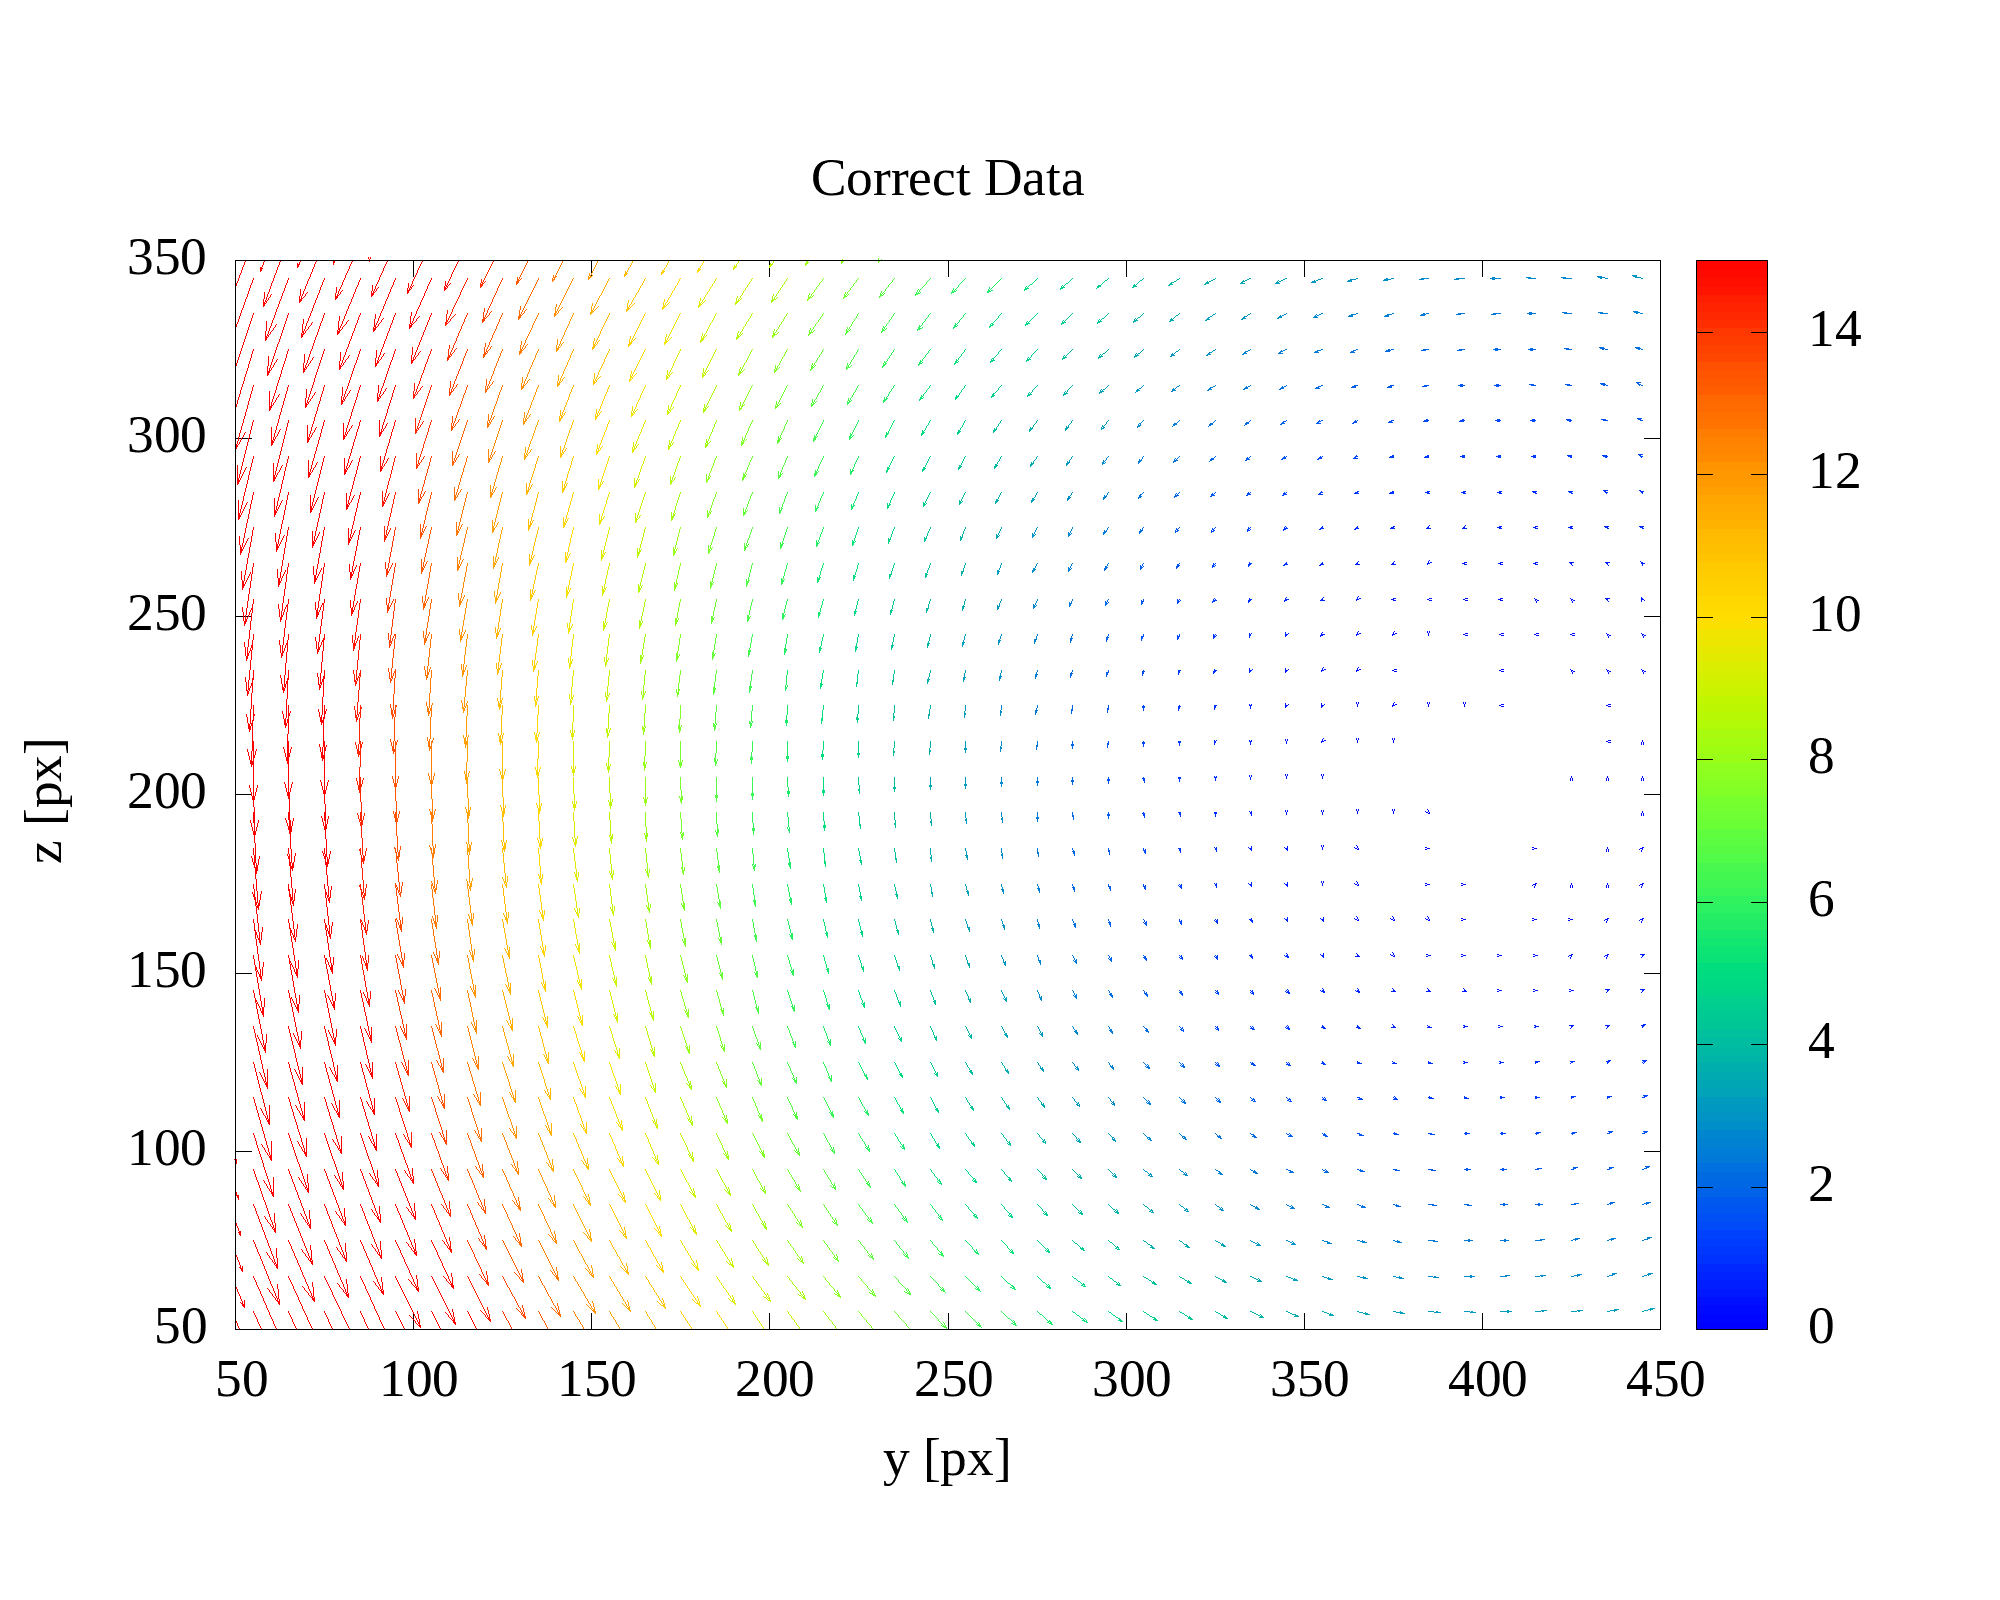
\includegraphics[width=80mm]{../images/correct.png}
    \caption{PIV:Correct Data}
  \end{center}
\end{figure}

\newpage

\subsection{正解データの作成条件}

\begin{table}[hbtp]
  \label{table:data_type}
  \caption{計算条件}
  \centering
  \begin{tabular}{ c c | r l}
    \hline
    壁の回転速度 & $\omega$ & 10                     & [deg/s]            \\ \hline
    動粘性係数   & $\nu$    & $1.004 \times 10^{-6}$ & [$\mathrm{m}^2$/s] \\ \hline
    計算対象位置 & $x$      & 7.000 + $\Delta T/2$   & [mm]               \\ \hline
  \end{tabular}
\end{table}

\noindent
$\blacksquare$ \textgt{速度式}
\begin{eqnarray*}
  \zeta &=& x \sqrt{\frac{\omega}{\nu}}\\
  u &=& r \omega F \left(\zeta\right)\\
  v &=& r \omega G \left(\zeta\right)\\
  w &=& \sqrt{\nu \omega} H \left(\zeta\right)
\end{eqnarray*}

\subsection{誤差評価式}
誤差評価を行うにあたり,今回は格子上に位置する
ベクトルの解析値と正解値の差と正解ベクトルの比を
をもとに算出した.

\begin{itemize}
  \item [$\blacksquare$]\textgt{データの定義}
        \begin{eqnarray*}
          A_{(i,j)},\;a_{y(i,j)},\;a_{z(i,j)} &:& 正解値\\
          V_{(i,j)},\;v_{y(i,j)},\;v_{z(i,j)} &:& シミュレーションの値
        \end{eqnarray*}
        \begin{eqnarray*}
          A_{(i,j)} &=& \sqrt{{a_{y(i,j)}^2} + a_{z(i,j)}^2}\\
          V_{(i,j)} &=& \sqrt{{v_{y(i,j)}^2} + v_{z(i,j)}^2}
        \end{eqnarray*}
        \item[$\blacksquare$]\textgt{誤差率の計算}
        \begin{eqnarray*}
          E_{y(i,j)} &=& \frac{\left| v_{y(i,j)} - a_{y(i,j)} \right|}{A_{(i,j)}} \times 100 \; [\%]\\
          E_{z(i,j)} &=& \frac{\left| v_{z(i,j)} - a_{z(i,j)} \right|}{A_{(i,j)}} \times 100 \; [\%]\\
          E_{(i,j)} &=& \frac{\left| V_{(i,j)} - A_{(i,j)} \right|}{A_{(i,j)}} \times 100 \; [\%]
        \end{eqnarray*}
\end{itemize}

\newpage

\subsection{誤差評価の結果}

\begin{figure}[htbp]
  \footnotesize
  \begin{center}
    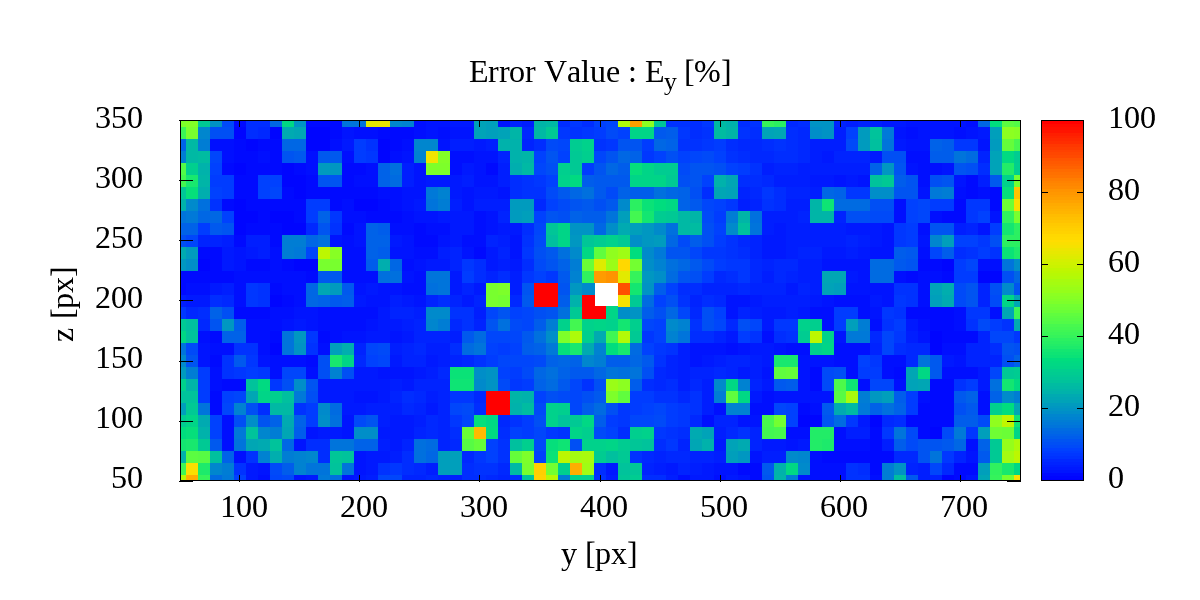
\includegraphics[width=80mm]{../images/error_y.png}
    \caption{Error Value : $\mathrm{E}_y$ [\%]}
    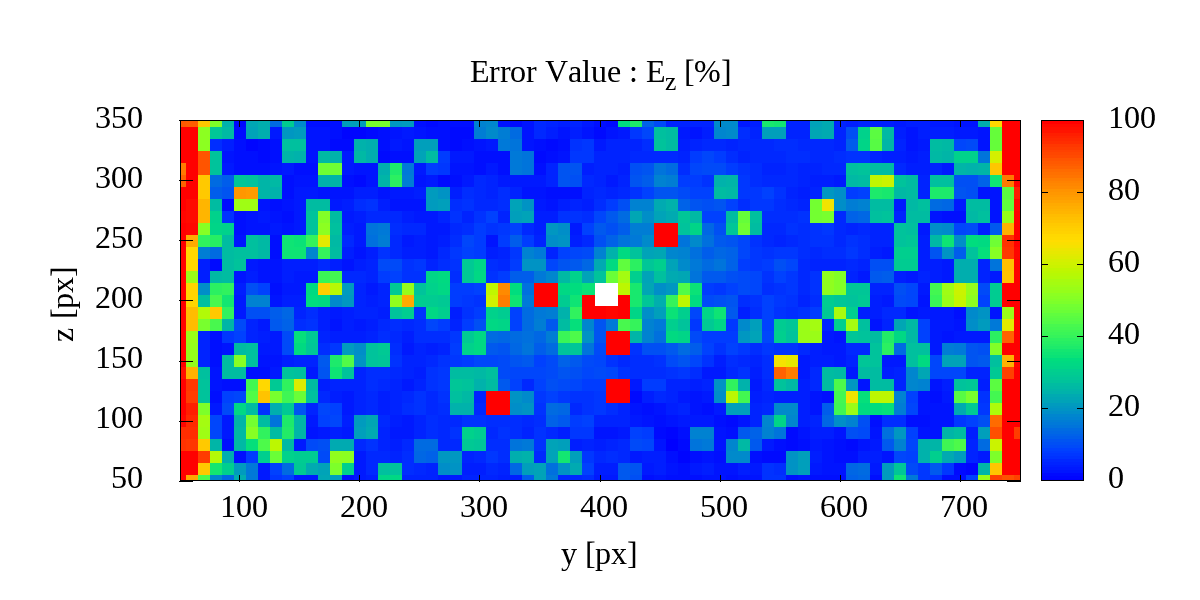
\includegraphics[width=80mm]{../images/error_z.png}
    \caption{Error Value : $\mathrm{E}_z$ [\%]}
    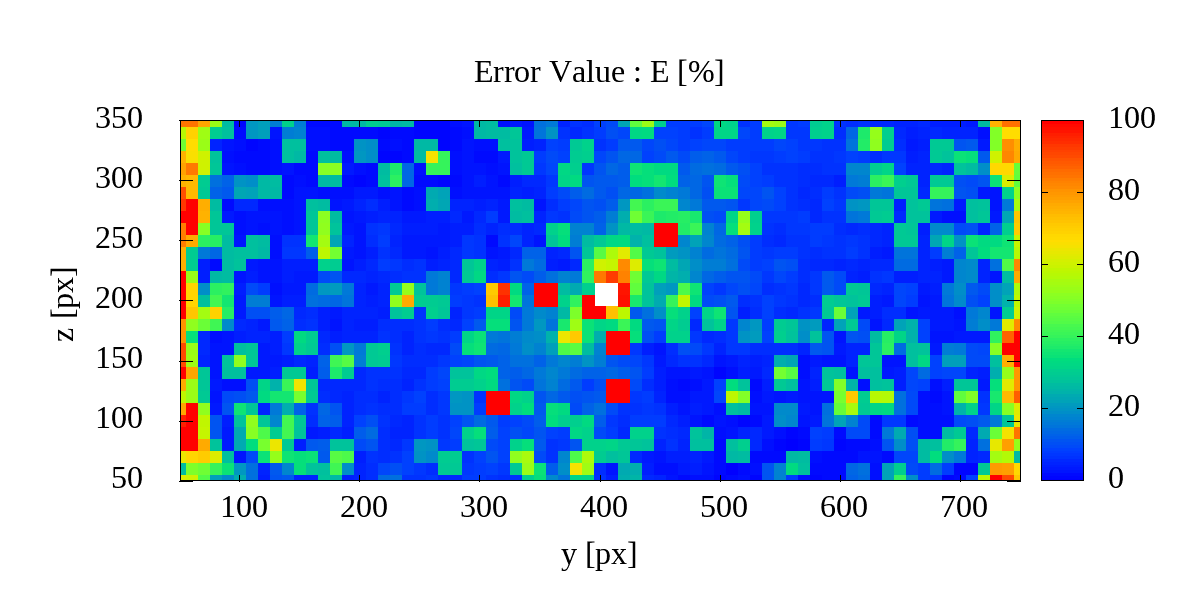
\includegraphics[width=80mm]{../images/error_value.png}
    \caption{Error Value : $\mathrm{E}$ [\%]}
  \end{center}
\end{figure}

\section{今後の予定}
\begin{itemize}
  \item 粒子密度の違いによる解析制度の比較
  \item 第51回 可視化情報シンポジウム 登録
  \item ASV17 原稿作成
  \item 4月度 共同研究報告会 資料作成
\end{itemize}

\end{document}